
\chapter{\'Etude du corpus de son \textit{ambiance}}
\label{chap:ambiance}
Dans ce chapitre, on étudie le comportement des différentes versions de la NMF, présentées dans le chapitre \ref{chap:nmf},  avec le premier corpus élémentaire \textit{Ambiance}. 
Dans un premier temps un rappel du corpus, des méthodes choisies et une présentation de la méthode de référence (ou \textit{baseline} en anglais). Puis les étapes menant à l'apprentissage du dictionnaire sont détaillées. Enfin les résultats des calculs, menés sur le corpus, sont présentés.


\section{Estimation du trafic routier}
Dans un premier temps, la composition du dictionnaire est décrite. Puis un résumé des facteurs expérimentaux impliqués est présenté.
\subsection{Rappel de la méthode employé}

Les étapes impliquées dans l'estimation du niveau sonore du trafic à partir de scènes sonores simulées sont d'abord rappelées. La Figure \ref{fig:rappel_estimateur} résume la démarche générale.

\begin{figure}[ht]
\centering
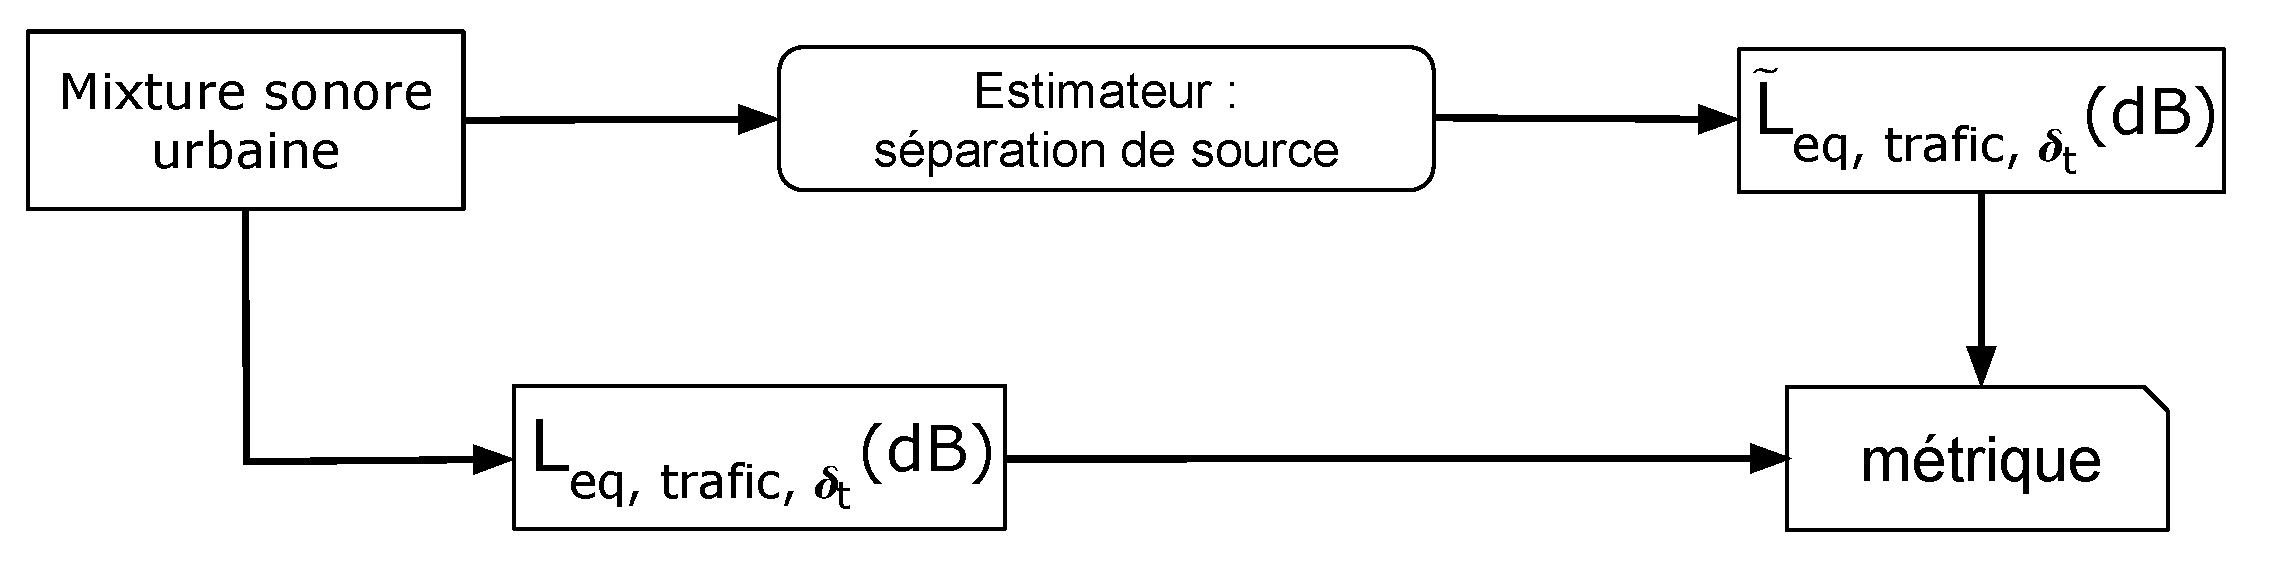
\includegraphics[width=.8\linewidth]{./figures/NMF/Bloc_diagram_estimateur_FR.pdf}
\caption{Diagramme en blocs dans l'estimation du niveau sonore du bruit de trafic}
\label{fig:rappel_estimateur}
\end{figure}

Le corpus de scènes sonore a été présenté dans \ref{} et est composé, pour rappel, de 6 sous-corpus : \textit{alert}, \textit{animaux}, \textit{climat}, \textit{humain}, \textit{transport}, \textit{mécanique}. Dans chaque sous-corpus, les 25 scènes sont dupliqué 5 fois où le niveau sonore du signal \textit{trafic} $L_{eq,trafic}$, qui inclut le bruit de fond routier ainsi que les évènements sonore \textit{passages de voitures}, est calibré par rapport au niveau sonore de la classe de son \textit{interférante}, $L_{eq,interferant}$, qui est composée des autres signaux sonores : 

\begin{equation}
TIR = L_{eq,trafic} - L_{eq,interferant}
\end{equation}

avec $TIR \in \lbrace -12,~-6,~0,~6,~12 \rbrace$. Ce corpus permet de tester les performances de la NMF et son comportement face à de tel mixtures sonores. En tout, 750 scènes d'une durée individuelle de 30 secondes (pour une durée totale de 6h30).
Chaque scène est ensuite soumis à l'estimateur qui détermine le niveau sonore du trafic estimé, $\tilde{L}_{eq,trafic}$. Pour chaque sous-corpus et valeur du TIR, les 25 niveaux estimés sont ensuite comparés à leur niveau sonore exacte, $L_{eq,trafic}$ au travers d'un calcul de métrique .
Cette métrique sera alors moyenné sur l'ensemble des sous-classes de sons par TIR : 

\begin{equation}
E = \frac{\sum_{i = 1}^6 METRIQUE_{i}}{6}
\end{equation}

Cette indicateur renseigne alors les performances de l'estimateur sur l'ensemble des sous-classes par TIR. Il est également possible de calculer cette indicateur sur l'ensemble des sous-classes et de TIR pour connaitre la combinaison de l'estimateur qui donne l'erreur la plus faible sur l'intégralité du corpus : 

\begin{equation}
E = \frac{\sum_{i = 1}^6 \sum_{j = 1}^5 METRIQUE_{i,j}}{6 \times 5}
\end{equation}

En vue d'obtenir une méthode qui puisse être le plus efficace sur l'ensemble du corpus sans connaissance a priori du $TIR$ ou de la sous-classe, c'est cette erreur qui sera d'abord observé.

\subsection{Estimateur baseline}
Pour comparer les performances de la NMF, un estimateur de référence (ou \textit{baseline} en anglais) est nécessaire. La baseline choisie est un filtre en fréquence passe-pas de fréquence de coupure $f_c$. Ce choix est justifié par la présence de composantes basses-fréquence (< 1000 Hz) dans les signaux trafic. 
Cet estimateur revient donc à supprimer toutes les composantes supérieures à $f_c$. Le signal obtenu est alors assimilé au signal trafic $\tilde{L}_{eq,trafic}$. 

La Figure résume les étapes intervenant pour cet estimateur.
Figure avec un spectrogramme complet et un spectrogramme coupé à 2000 Hz et ensuite niveau sonores.

Les fréquences de coupures choisies sont alors $f_c = \lbrace 100, 250, 500, 1k, 2k, 5k, 10k, 20k \rbrace$ Hz. Le cas où $f_c = 20 kHz$ correspond finalement au cas où aucun traitement du signal n'est réalisé sur les fichiers audio et traduit le cas où la question de la présence des sources sonores qui composent le signal n'est pas considérée.

\subsection{Estimateur basé sur la NMF}
Ce second estimateur est basé sur la NMF présenté dans le chapitre \ref{chap:nmf}. 
La Figure \ref{fig:nmf_ambiance} résume les différentes étapes présentes dans la NMF.

\begin{figure}[ht]
\centering
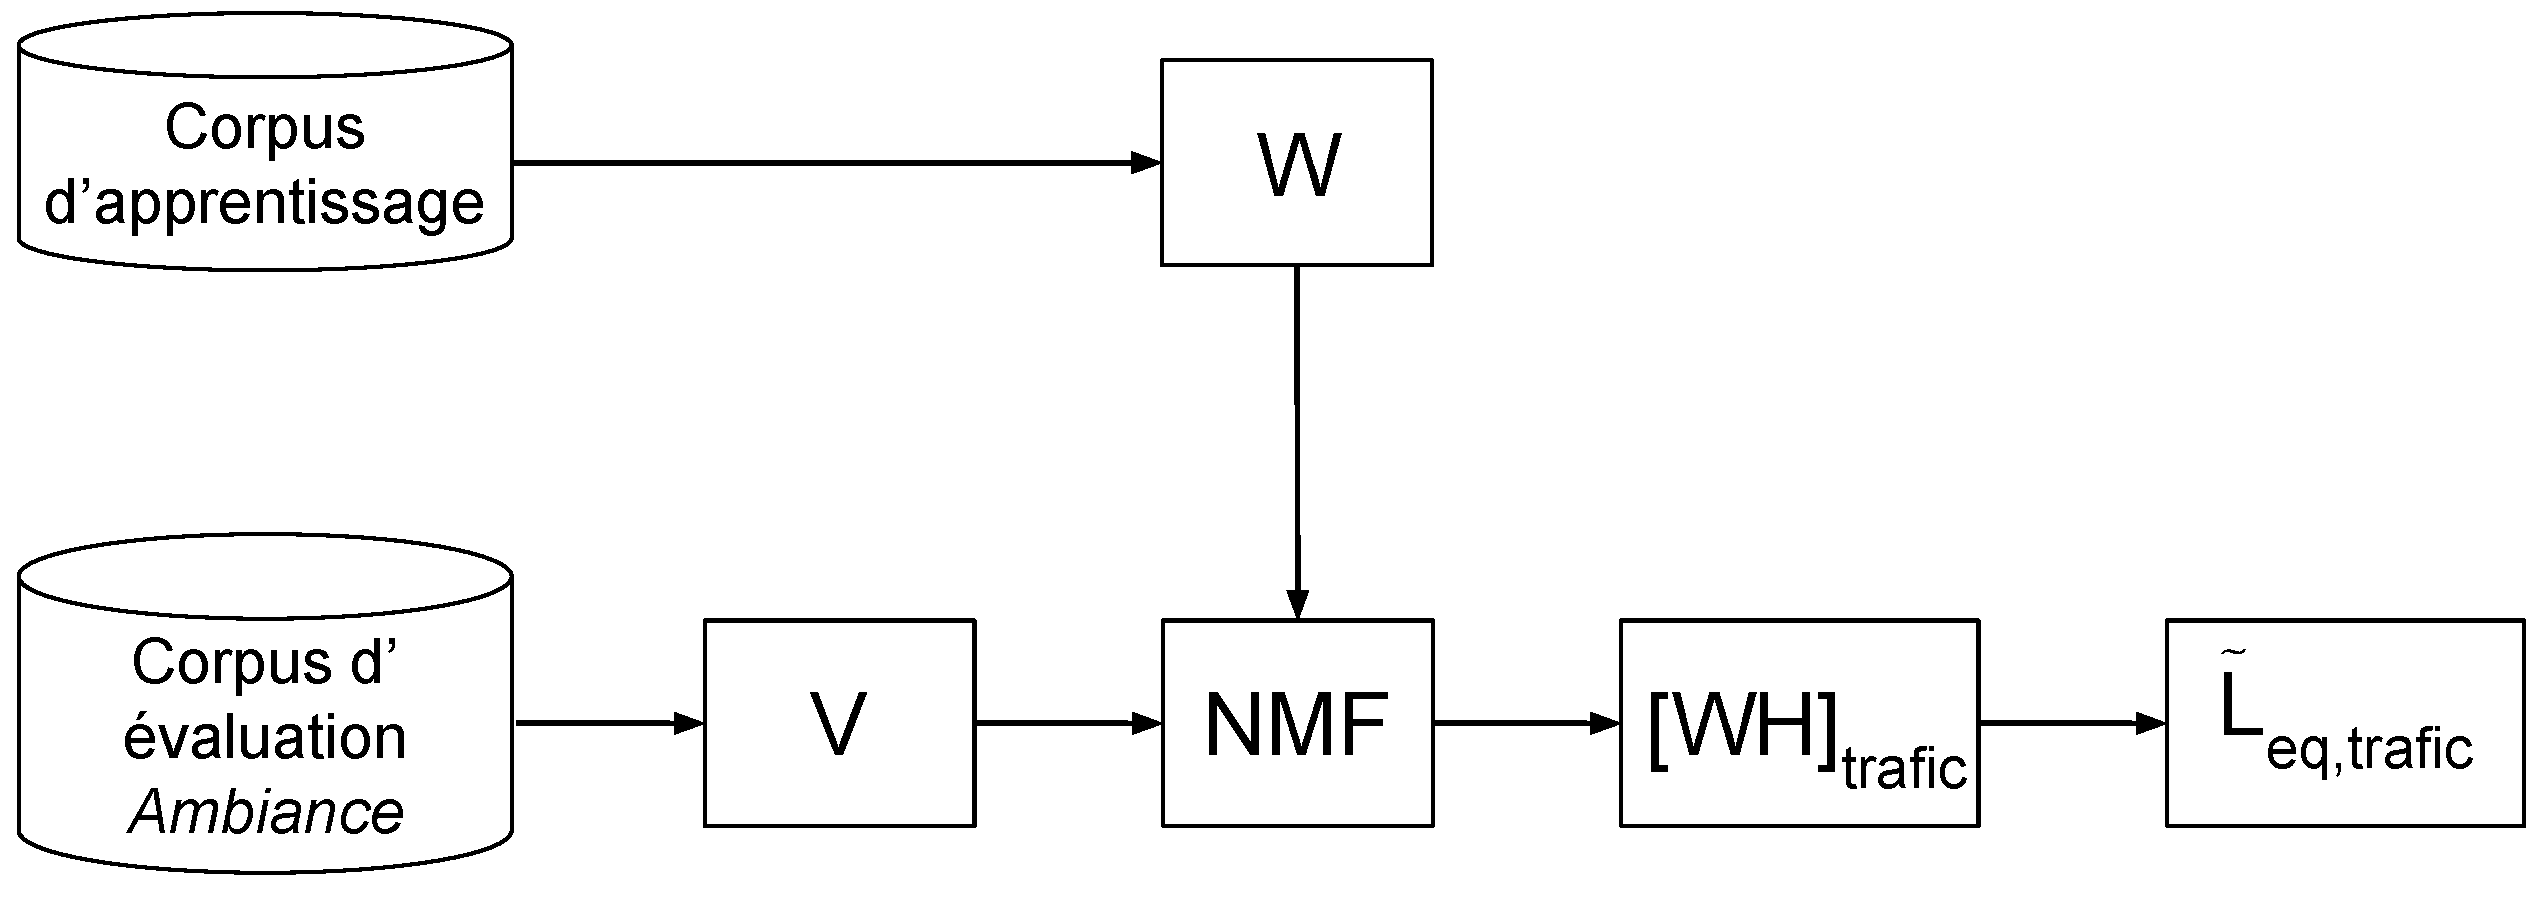
\includegraphics[width=0.7\linewidth]{./figures/NMF/NMF_ambiance.pdf}
\caption{Diagramme en blocs de l'estimateur NMF sur le corpus élémentaire \textit{Ambiance}}
\label{fig:nmf_ambiance}
\end{figure}


\subsubsection{Constitution du dictionnaire}
Dans un premier temps, le dictionnaire $\mathbf{W}$ est construit, à partir du corpus de référence, composé des fichiers audio des passages des voitures enregistrés des voitures Renault Scénic et Dacia Sandero sur la piste d'essais. Ces 53 échantillons audio issus des enregistrements ne sont pas ceux utilisés dans la création des scènes sonores afin d'éviter tout problème de sur-apprentissage.

\begin{figure}[hbtp]
\centering
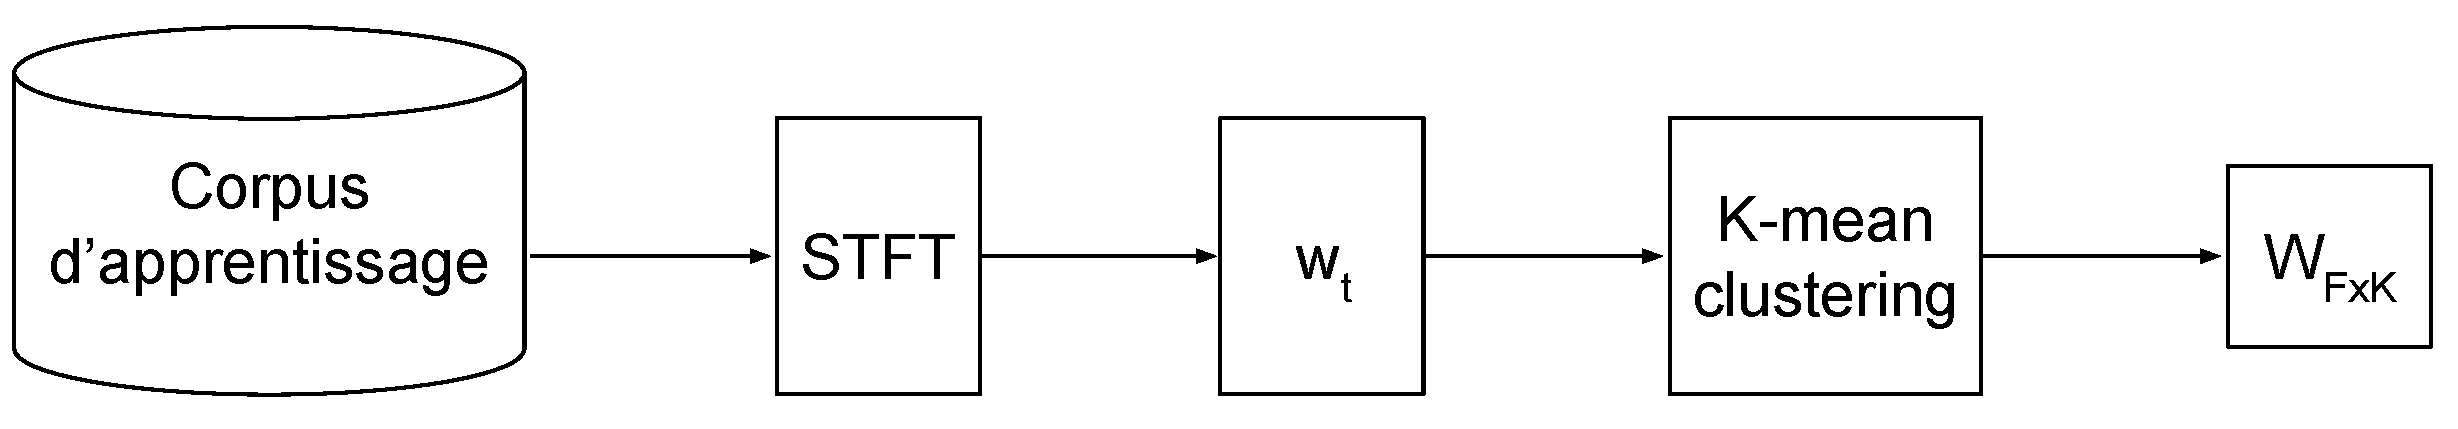
\includegraphics[width=.9\linewidth]{./figures/NMF/creation_dictionaire.pdf}
\caption{Diagramme en blocs de la création du dictionnaire}
\label{fig:creation_W}
\end{figure}


La constitution du dictionnaire est réalisée en trois étapes, résumée dans le diagramme en bloc en Figure \ref{fig:creation_W} : 
\begin{itemize}
\item chaque fichier audio est représenté au travers d'un spectrogramme, obtenu par une STFT (nombre de point $w = 2^{12}$ avec 50 $\%$ de recouvrement). Cette première étape permet de représenter chaque échantillon audio, de durée différente, avec le même nombre de point en fréquences.
\item Chaque spectrogramme est ensuite découpé en plusieurs trames de largeur $w_t \in \lbrace 0,5,~ 1,~ 2~\rbrace$ seconde. Dans chaque trame la valeur efficace (ou valeur \textit{rms} en anglais) sur chaque trame fréquentiel est calculé. Cet étape a pour but d'obtenir différents représentation des spectrogrammes initiaux qui ont un description plus ou moins fine du contenu spectrale. Pour $w_t = 0,5$, on obtient une description plus fine que dans le cas où $w_t = 2$. Les détails de cette étape est décrit en Figure \ref{fig:decoupe_W}.
\item Enfin, l'opération précédente générant un grand nombre de fichier (2218 pour $w_t$ = 0,5 s, 505 éléments pour $w_t$ = 2 s), un algorithme de clustering $K$-mean est appliqué en vue de réduire ce nombre, d'éviter la présence d'informations redondates et de fixer le nombre d'éléments à $K = \lbrace 25,~50,~100,~200 \rbrace$. Les $K$ centroïdes déterminés sont alors les éléments qui composent le dictionnaire $\mathbf{W}$.
\end{itemize}

En plus de ces étapes, on ajoute un cas où la valeur \textit{rms} est calculé sur l'ensemble des spectrogrammes ($w_t = all$). En cela, des 53 fichiers audio, 53 spectres sont générés. Cette opération permet de baser la construction du dictionnaire sur des enveloppe spectrale et moins sur une description fine des spectres. Ces 53 spectres sont également soumis à l'algorithme de clustering mais avec cette fois, $K \in \lbrace 25,~ 50 \rbrace$. En tout, c'est 14 versions différentes du dictionnaire qui sont réalisées ($4\times 3 + 1 \times 2$).

\begin{figure}[hbtp]
\centering
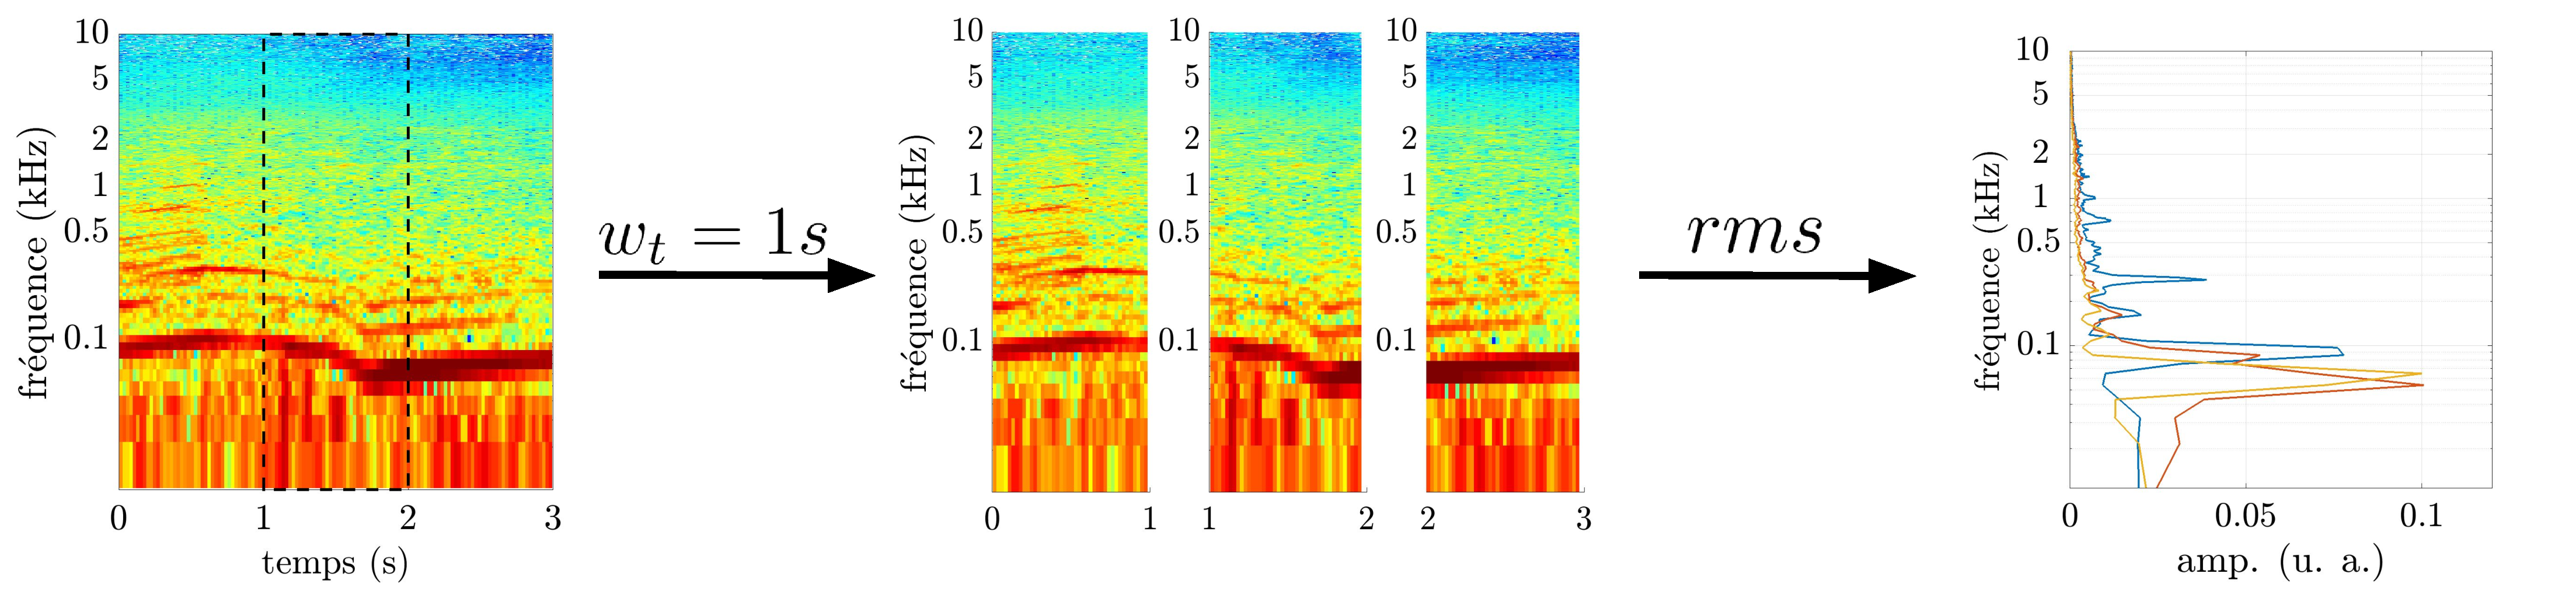
\includegraphics[width=.9\linewidth]{./figures/NMF/dictionaire_frame_FR.pdf} 
\caption{Création des éléments sur un extrait de 3 secondes du passage d'une voiture pour une largeur de la trame temporelle $w_t$ de 1 seconde. À gauche le spectrogramme du signal audio avec, en pointillés, une fenêtre de découpe de largeur $w_t$. Le signal est ainsi découpé en trois parties dont les valeurs \textit{rms} sont ensuite calculés. }
\label{fig:decoupe_W}
\end{figure}

\subsubsection{Réalisation de la NMF}

Ces dictionnaires $\mathbf{W}$ sont chacun soumis à l'estimateur NMF. Cette estimateur est lui-même basé sur plusieurs version de la NMF décrit précédemment (voir partie \ref{}) : la NMF supervisée (NMF-SUP), semi-supervisée (NMF-SS) et Initialisée-seuillée (NMF IS). Dans le cas de la NMF-SS, le dictionnaire fixe $W_s$ correspond aux dictionnaires générés, le nombre d'éléments du dictionnaire libre $W_r$ est alors fixé à 2 ($J = 2$). Dans le cas de la NMF-IS, les dictionnaires $W$ correspondent aux dictionnaires initiaux $W_0$ qui seront ensuite mis à jours.

Pour chacun version de la NMF, 3 $\beta$-divergences sont utilisées : la distance Euclidienne ($\beta = 2$), équation \ref{}, la divergence de Kullback-Leibler ($\beta = 1$), équation \ref{}, et la divergence d'Itakura-Saïto ($\beta = 0$), equation \ref{}. Pour chaque méthode, XXX itérations sont réalisées. 

Dans le cas de la NMF-SUP et NMF-SS, les niveaux sonores sont extrait directement après avoir réalisé les 200 itérations. Pour la NMF-IS, le dictionnaire obtenu est soumis à une étape de classement. L'influence de plusieurs paramètres présentés dans la partie \ref{} sur l'estimation du trafic est observée : 

\begin{itemize}
\item la représentation de la distance $D_{\theta}(\mathbf{W_0}\Vert \mathbf{W})$ (linéaire ou bien exprimé au travers d'une fonction sigmoïde),
\item le type de seuillage appliqué (dur ou \textit{firm}),
\item les valeurs des différents seuils respectifs ($t_h$ pour le seuillage dur et $t_{f,1/2}$, les deux valeur seuils pour le seuillage \textit{firm}). Des études préliminaires ont permis de réduire les valeurs limites de ces seuils à $t_h \in \lbrace 0.30~0.70 \rbrace$, $t_{f,1} \in \lbrace 0.20~0.55 \rbrace$ et $t_{f,2} \in \lbrace 0.35,~0.65 \rbrace$, chacune étant défini avec un pas de 0,01.
\end{itemize}


\'Egalement, une représentation en bande tiers-d'octave a été choisie pour $\mathbf{W}$ et $\mathbf{V}$. Cette représentation a plusieurs intérets : 

\begin{itemize}
\item par son échelle logarithmique, elle permet de mieux décomposer les basses fréquences que les hautes fréquences. On permet alors de mieux focaliser la reconstruction du signal vers les bandes de fréquences d'intérêts.
\item Cette représentation est également couramment utilisée dans le domaine de l'acoustique urbaine et environnementale, à la différence des MFCC. En vue des applications prévue de ces outils (amélioration de la cartographie, estimation des sources sonores urbaines), c'est une représentation plus adaptée.
\item enfin, le nombre de bande étant réduites ($F_{1/3} = 29$), la manipulation des matrices est plus rapide qu'avec des bandes fines et donc permet un gain en temps de calculs.
\end{itemize}

FIGURE SPECTRE LIN ET TIERS D'UNE VOITURE

\subsubsection{Résumé des facteurs expérimentaux}

De nombreux facteurs expérimentaux sont présents dans cette expérience, chacun ayant des différentes modalités. Le Tableau \ref{tab:experimental_factorsNMF_ambiance} résume l'ensemble de ces paramètres.

\begin{table*}[t]
\centering
\caption{Facteurs expérimentaux et leur modalité utilisé pour le corpus \textit{Ambiance}.}
\begin{tabularx}{17.5cm}{L{3cm}@{}C{12cm}@{}C{2cm}@{}}
	\hline
    \textbf{\begin{tabular}[c]{@{}l@{}}facteur \\ expérimentaux \end{tabular}} & \textbf{modalités} & \begin{tabular}[c]{@{}C{2cm}@{}}\textbf{nombre de}\\ \textbf{modalité}\end{tabular}\\ \toprule
\end{tabularx}

\begin{tabularx}{17.5cm}{L{2.8cm}@{}@{}C{2cm}@{}@{}C{2cm}@{}@{}C{2cm}@{}@{}C{2cm}@{}@{}C{2cm}@{}@{}C{2.2cm}@{}C{2cm}}
\rowcolor[HTML]{C0C0C0}
   environnement sonore (kHz) & alerte & animaux & climat &  humain & transport & mécanique & 6\\
\end{tabularx}

\begin{tabularx}{17.5cm}{L{2.8cm}@{}@{}C{2.2cm}@{}@{}C{2.2cm}@{}@{}C{2.2cm}@{}@{}C{2.2cm}@{}@{}C{2.2cm}@{}C{2cm}}
\rowcolor[HTML]{C0C0C0}
   $TIR$ (dB) & -12 & -6 & 0 & 6 & 12 & 5\\
\end{tabularx}

\begin{tabularx}{17.5cm}{L{3cm}@{}C{3cm}@{}@{}C{3cm}@{}@{}C{3cm}@{}@{}C{3cm}@{}C{2cm}@{}}
  \textbf{method} & filtre passe bas & NMF SUP & NMF SEM & NMF IS & 4\\
\end{tabularx}

\begin{tabularx}{17.5cm}{L{3cm}@{}@{}C{2cm}@{}@{}C{2cm}@{}@{}C{2cm}@{}@{}C{2cm}@{}@{}C{2cm}@{}@{}C{2cm}@{}C{2cm}@{}}
\rowcolor[HTML]{C0C0C0}
   $\mathbf{f_c}$ (kHz) & 0.5 & 1 & 2 &  5 & 10 & 20 & 6\\
\end{tabularx}

\begin{tabularx}{17.5cm}{L{3cm}@{}C{3cm}@{}@{}C{3cm}@{}@{}C{3cm}@{}@{}C{3cm}@{}C{2cm}@{}}
    $\mathbf{w_t}$ (s)& 0.5 & 1 & 2 & \textit{all} & 4\\
\end{tabularx}

\begin{tabularx}{17.5cm}{L{3cm}@{}C{3cm}@{}@{}C{3cm}@{}@{}C{3cm}@{}@{}C{3cm}@{}C{2cm}@{}}
	\rowcolor[HTML]{C0C0C0}
    $\mathbf{K}$ & 25 & 50 & 100 & 200 & 4\\
\end{tabularx}

\begin{tabularx}{17.5cm}{L{3cm}@{}C{4cm}@{}@{}C{4cm}@{}@{}C{4cm}@{}C{2cm}@{}}
   $\mathbf{\beta}$ & 0 & 1 & 2 & 3\\
\end{tabularx}

\begin{tabularx}{17.5cm}{L{3cm}@{}C{6cm}@{}@{}C{6cm}@{}C{2cm}@{}}
	\rowcolor[HTML]{C0C0C0}
   représentation & linéaire & sigmoïde & 2\\
\end{tabularx}

\begin{tabularx}{17.5cm}{L{3cm}@{}C{12cm}@{}C{2cm}@{}}
	seuillage dur $\mathbf{t_h}$ & de 0.30 à 0.60 avec un pas de 0.01 & 31\\
\end{tabularx}

\begin{tabularx}{17.5cm}{L{3cm}@{}C{12cm}@{}C{2cm}@{}}
	\rowcolor[HTML]{C0C0C0}
   seuillage firm $\mathbf{t_{f,1}}$ & de 0.20 à 0.55 avec un pas de 0.01 & 36\\
\end{tabularx}

\begin{tabularx}{17.5cm}{L{3cm}@{}C{12cm}@{}C{2cm}@{}}
   seuillage firm $\mathbf{t_{f,2}}$ & de 0.35 à 0.65 avec un pas de 0.01 & 31\\
   \bottomrule
\end{tabularx}
\label{tab:experimental_factorsNMF_ambiance}
\end{table*}

Dans le cas de la NMF SUP et SS, selon les 14 versions du dictionnaire et les 3 valeurs de $\beta$, le nombre de combinaison de modalité est de 42 (14 dict. $\times$ 3 $\beta$ $\times$ 6 sous-classes $\times$ 8 $TIR$).
Dans le cas de la NMF IS, ce nombre est beaucoup plus élevé en raison des nombreuses valeurs seuils qui sont possibles.

Les calculs sont réalisés sous le logiciel Matlab, avec l'aide de l'outil expLanes\footnote{\url{http://mathieulagrange.github.io/expLanes/}} qui permet la réalisation d'expériences numérique, de gérer la distribution des nombreux facteurs expérimentaux et leur modalités et de collecter les nombreux résultats générés.

\section{Résultats}

\subsection{Performance de l'estimateur \textit{baseline}}

Les résultats issus de l'estimateur baseline sont d'abord présentés. Dans un premier temps, on résumé dans le Tableau les erreurs moyennes émises pour chaque filtre sur l'ensemble du corpus. Les erreurs moyennées sur l'ensemble des sous-corpus par TIR est également résumés. 

\begin{table}[]
\centering
\caption{Erreur XXX de l'estimateur \textit{baseline} selon $f_c$ sur l'ensemble du corpus \textit{Ambiance} et pour chaque TIR}
\label{tab:resuls_ambiance_filtre}
\resizebox{\textwidth}{!}{%
\begin{tabular}{lcccccc}
$f_c$ (Hz) & MAE & -12 & -6 & 0 & 6 & 12 \\ \toprule
100 &  &  &  &  &  &  \\
\rowcolor[HTML]{C0C0C0}
250 &  &  &  &  &  &  \\
500 &  &  &  &  &  &  \\
\rowcolor[HTML]{C0C0C0}
1k &  &  &  &  &  &  \\
2k &  &  &  &  &  &  \\
\rowcolor[HTML]{C0C0C0}
5k &  &  &  &  &  &  \\
10k &  &  &  &  &  &  \\
\rowcolor[HTML]{C0C0C0}
20k &  &  &  &  &  & \\ \bottomrule
\end{tabular}}
\end{table}


\subsection{Résultats de la NMF}

\subsection{Résultats de la NMF-SUP et NMF-SS}

\subsection{Résultats de la NMF-IS}


\begin{itemize}


\item résultats
\begin{itemize}
\item mae générale (filtre VV, supervisé, semi-supervisé, seuillé VV)
\item mae pour chaque TIR et chaque ambiance (filtre VV, supervisé, semi-supervisé, seuillé VV)
\item allure des courbes Lp,1s pour TIR -12 et 12 (supervisé, semi-supervisé, seuillé) dans deux cas extrêmes, y'a des fois ou ça marche moins notamment avec la météo mais ça c'est moins grave (on a des capteurs, on peut les mettre à part, à voir si ce n'est que l'orage)
\item fonction cost (supervisé, semi-supervisé, seuillé)
\item allure des 2 éléments dans Wr
\item distance $w_0$ et $w$
\end{itemize}
\end{itemize}





%\end{document}
